{In this problem, you will use your functions from the previous problems, running them with specific numeric input(s).
\begin{enumerate}
\item Run your \cour{ProjMotion} function for 0 to 30 seconds in increments of 0.5 seconds and use the output to plot \cour{time} versus \cour{height}. Use the output of the function (and appropriate Matlab functions) to figure out at what time the object starts to fall back to the ground.\\
\item Run your currency conversion function to give the output from an input \cour{dollars}) ranging from 0 to 100 in increments of 5.\\
\item Run your \cour{plotlines} function with the inputs \cour{[1, 1]} and \cour{[2, 4;5, 6]}.  Your output should look like\\
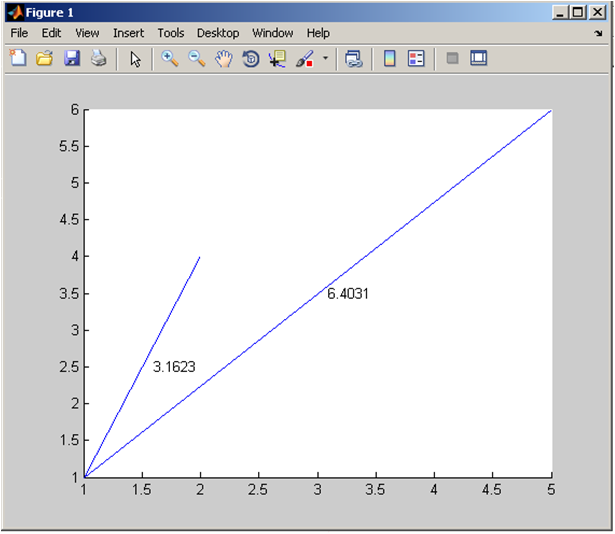
\includegraphics[scale=.75]{figures/matlab_functionplot1.png}
\item Run your \cour{RemRow} function with inputs \cour{[1 2 3; 4 5 6; 7 8 9]} and \cour{2}. The output should be the matrix with the 2nd row removed.\\
\item Run your \cour{RemCol} function with inputs \cour{[1 2 3; 4 5 6; 7 8 9]} and \cour{2}. The output should be the matrix with the 2nd columns removed.\\
\item Run your time conversion function to give the conversion for \textrm{1,000} seconds, \textrm{1,000,000} seconds and \textrm{1,000,000,000} seconds.  
\end{enumerate}}
{}